\documentclass[10pt,twocolumn]{article} 
\usepackage{simpleConference}
\usepackage{times}
\usepackage{graphicx}
\usepackage{amssymb}
\usepackage{url,hyperref}
\usepackage{xcolor}
\usepackage{mdframed}

\begin{document}

\title{CS670 Project Proposal\\Fraudulent Lockstep Behavior Detection}

\author{
Team Name: \textbf{End of Fraud}\\[2ex]
Team Members \small{(alphabetically ordered)}:\\[1ex]
Majid Alfifi, Parisa Kaghazgaran,  Xing Zhao
}

\maketitle
%\thispagestyle{empty}

%\begin{abstract}
%   This is a simple sample of a document created using \LaTeX
%   (specifically pdflatex)
%   that includes a figure from the Vergil visual editor for Ptolemy II
%   that was created by printing to the Acrobat Distiller to get a PDF file.
%   It also illustrates a simple two-column conference paper style,
%   and use of bibtex to handle bibligraphies.
%\end{abstract}
%

\section{Introduction}
 
% An article style is separated into sections and subsections with 
%   markup such as this.  Use \section*{Principles} for unnumbered sections.

\begin{figure}[!b]
%\begin{mdframed}
  \begin{center}
    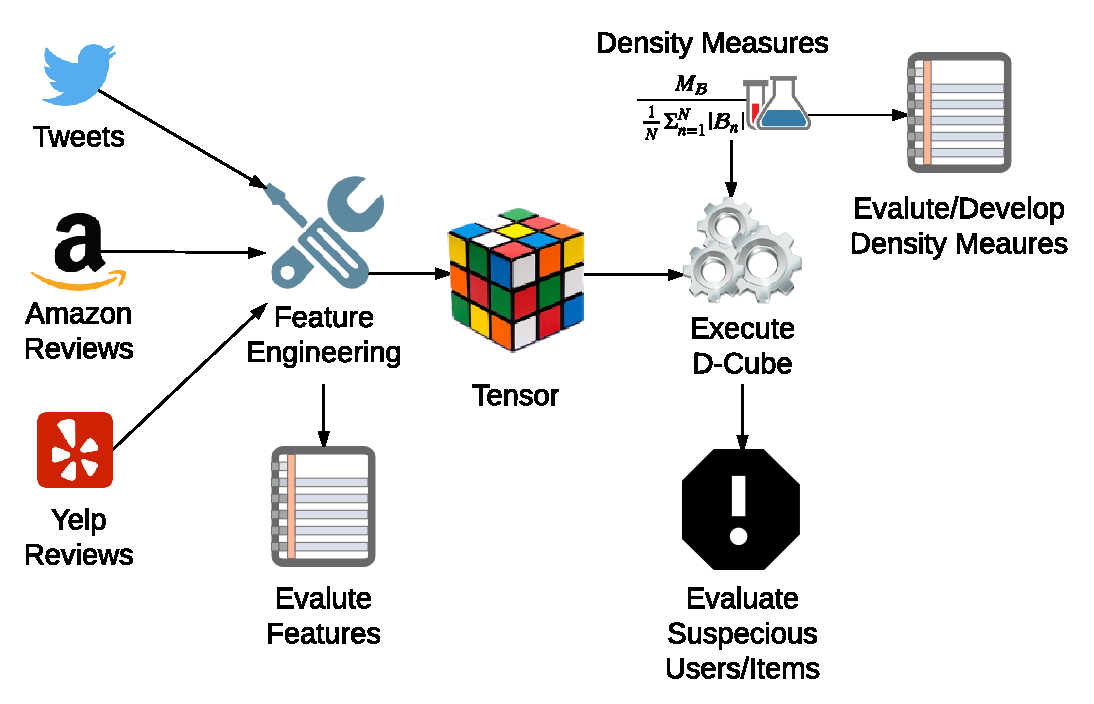
\includegraphics[width=3.5in]{figure.pdf}
  \end{center}
%\end{mdframed}
  \caption{\small Project plan: \emph{Feature engineering} will help find the most useful dimensions to use in the Tensor to enable better suspicious blocks detection. \emph{Density measures} experiments will evaluate different existing measures in addition to custom measures that might be suitable for our own datasets.}
  \label{fig:process}

\end{figure}

How can we detect if a politician has purchased fake followers on Twitter or if a product's reviews on Amazon are not genuine?

A common method has been to represent \emph{users} and \emph{items} as a matrix where in the simplest case a cell can take on a binary value of 1 or 0 indicating whether there is a relationship between the corresponding user and item or not. The problem can then be transformed to finding dense regions in this matrix \cite{hooi2016fraudar}. Moreover, this method has been lately extended from matrix to tensor representation to incorporate more dimensions from the domain such as timestamp, Twitter followers count, or number of stars of an Amazon product \cite{shin2016m} \cite{shin2017d}. Extraordinary dense blocks in the tensor correspond to groups of users with lockstep behaviors both in the items they relate to and along the additional dimensions (for example, multiple users reviewing the same products at the exact same time). A scalable MapReduce-based implementation \textbf{D-Cube}\footnote{\href{https://github.com/kijungs/dcube}{https://github.com/kijungs/dcube}} was also provided by \cite{shin2017d} which we intend to evaluate and build on in this project.



\section{Project Goals}

As illustrated in Figure \ref{fig:process}, we intend to use an existing MapReduce-based implementation of the D-Cube algorithm (Section 3.3 in \cite{shin2017d}) on our own datasets with two main goals:
\begin{enumerate}
	\item \textbf{Feature engineering}: we will explore the effectiveness of different dimensions in each of our datasets in detecting fraudulent lockstep behavior; hopefully also informing our own research.
	\item \textbf{Empirical study of density measures}: we aim to experiment and build on several density measures defined in \cite{shin2017d} (Section 2.2) and its foundations previously laid in \cite{jiang2015general} and potentially propose our own flexible density measures that take into account weights of different features in different datasets. For example, In Amazon dataset, is the temporal dimension more informative than product rating?
\end{enumerate}

\section{Datasets}
We intend to apply and experiment with the D-Cube algorithm on the following datasets:
\begin{itemize}
\item \textbf{Twitter dataset:} 9 billion tweets of which 2 billion are from eventually suspended users. This dataset was obtained through an industry contact.

\emph{Questions:} Can we identify tweets/users tampering with hashtags in efforts to promote/undermine discussions in those hashtags? How do those suspicious tweets temporally differ from ordinary tweets (timestamp dimension)? Can we identify users hired to attack other users by continuously replying to their tweets casting doubt on their cause? etc. 

\item \textbf{Amazon dataset:} About 500,000 Amazon reviews of which 21,000 are from crowdturfing products and the rest are from activity history of reviewers who wrote a review under these products. This dataset was collected from Amazon.com

\emph{Questions:} Can we find the hidden relation among reviewers in Amazon who aim to promote a product by writing fake reviews using additional dimensions such as temporal, rating and so on.

\item \textbf{Yelp dataset:} 4.1M reviews by 1M users for 144K businesses. This dataset is made available for researchers by Yelp\footnote{\href{https://www.yelp.com/dataset}{https://www.yelp.com/dataset}}.

\emph{Questions:} Can we identify fraud users (e.g. who gave the reviews for multiples businesses in a same day) who were hired to give fake reviews to a business? What are their behaviors (e.g. their average ratings) in their reviews? What kind of features (e.g. geo-location, business type, etc.) do businesses reviewed by fraud users have?
\end{itemize}

\section{Evaluation}
The D-Cube paper \cite{shin2017d} evaluates performance of the algorithm on synthetic data (i.e. by injecting random dense blocks in the tensor). However, we intent to provide a more realistic evaluation of the quality of each dense block (or blocks) found by D-Cube as follows:

\begin{itemize}
	\item \textbf{Twitter dataset:} How many of the suspicious users found were eventually suspended or deleted by Twitter? What is the size of the intersection between top hashtags used by suspended users and hashtags identified by D-Cube?
	\item \textbf{Amazon dataset:} How many of the suspicious products found were actually for products known to have explicitly recruited  reviewers on crowdsourcing websites?
	\item \textbf{Yelp dataset:} How many of the suspicious reviews found were filtered by Yelp?
\end{itemize}

In addition, we will sample few hundred users and items from each block we find and investigate them manually using our own domain knowledge of how fraudulent behavior in each domain looks like.


%The paper [2] defines several density measures appropriate for anomaly detection (Section 2.2). We aim to build on those functions and propose a flexible density measure which gives different weights to different features (e.g., In Amazon temporal features are more informative than rating).  
 
\section{Tools/Resources}
In addition to all the tools and methods we learned in the course, we will use a local Hadoop cluster to run the D-Cube algorithm.

\section{Project Outcome}

\begin{itemize}
	
	\item Evaluation of the accuracy of dense suspicious blocks found in each dataset.
	\item Evaluation of different dimensions useful for each dataset. 
	\item Evaluation of different density measures for each dataset.
	\item (Optional) New density measures that are more suitable to the nature of the  datasets we study.
\end{itemize}

\bibliographystyle{abbrv}
\bibliography{refs}
\end{document}
